\section{Results}

Przetestuje 4 kombinacje modeli, ze zmienioną funckją kosztu

\add{dodać krótki opis modeli i może dla czego softmax}

W tabeli \ref{table:results} zostały przedstawione wyniki dla czterech kombinacji modeli oraz parametrów. Wartości liczbowe opisują najlepsze AUC ROC podczas uczenia wraz z odpowiadającą epoką. Jak widać w tym zestawieniu najlepiej wypadły podstawowe modele VAE.

\begin{table}[h!]
	\centering
    \begin{tabular}{ l | c }
    \toprule
    Model 			& Best ROC AUC \\ \midrule
    VAE 				& 0.68 (1) \\
    VAE + Softmax 	& 0.68 (1) \\
    C-VAE 			& 0.59 (1) \\
    C-VAE + Softmax & 0.67 (1) \\
    \bottomrule
    \end{tabular}
    \caption{My table}
	\label{table:results}
\end{table}
\improvement{Dodać z-dim}

\section{Analysis}

Zajmę się analizą modelu w wersji VAE + Softmax. Na wykresie \ref{fig:soft_vae} przedstawione są koszty, ich rozkłady, przykłady rekonstrukcji oraz krzywa ROC. Ciekawie wyglądają te dwa zauważalne ogony na wykresie. Postaram sie lepiej przyjrzeć ich specyfice. 

Pierwszym pomysłem jest, żeby sprawdzić rozkład obrazków w zależności od ich jasności, czyli łącznej sumy pikseli. Ciemne obrazki defiuniuje jako te o niskiej sumie, a jasne o wysokiej. Na rysunku \ref{fig:soft_vae_th} zaznaczyłem negatywne obrazki, dla których suma <= 50 oraz pozytywne obrazki z sumą co najmniej 150. Zaznaczone śa one odpowiednio zielonym i czerwonym kolorem na wykresie. Jak widać po rozkładach składają się one na dokładnie te 2 separowalne ogony. Wniosek z tego jest następujący. Na podstawie tego modelu możemy odesparować jedynie najciemniejsze i najjaśniejsze obrazki z obydwu klas. W takim razie model nie robi nic nadzwyczajnego. Wystarczy przyjrzeć się histogramowi na rysunku \ref{fig:pixels_hist} z zaznaczonymi progami. One już bardzo dobrze separują te klasy. 

\begin{figure}[h!]
    \centering
    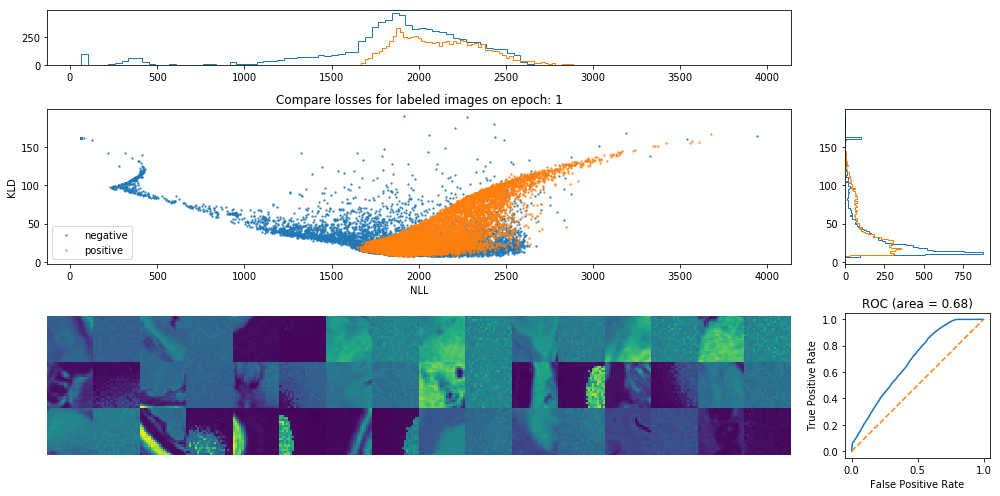
\includegraphics[width=1.0\textwidth]{images/soft_vae}
    \caption{}
    \label{fig:soft_vae}
\end{figure}

\begin{figure}[h!]
    \centering
    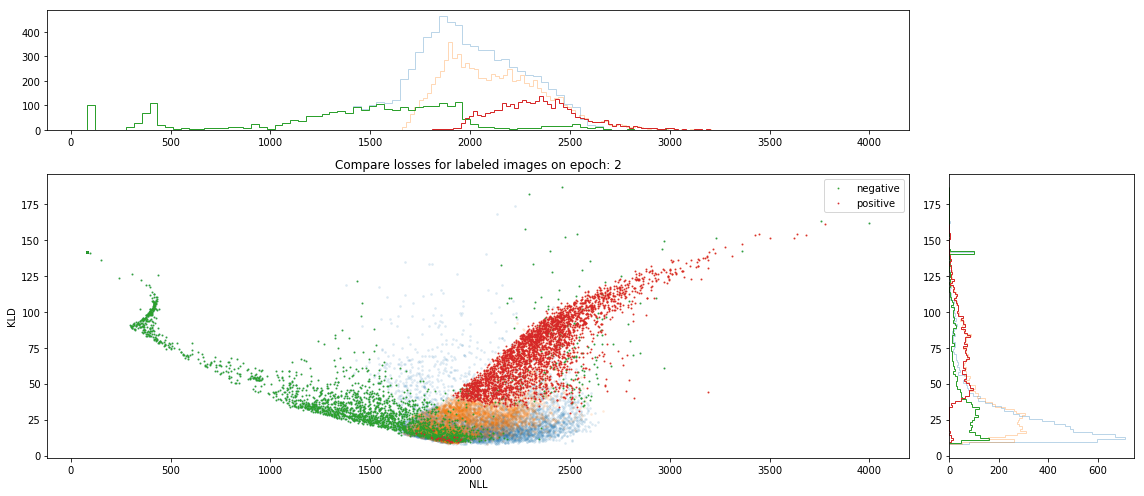
\includegraphics[width=1.0\textwidth]{images/soft_vae_th}
    \caption{}
    \label{fig:soft_vae_th}
\end{figure}

\begin{figure}[h!]
    \centering
    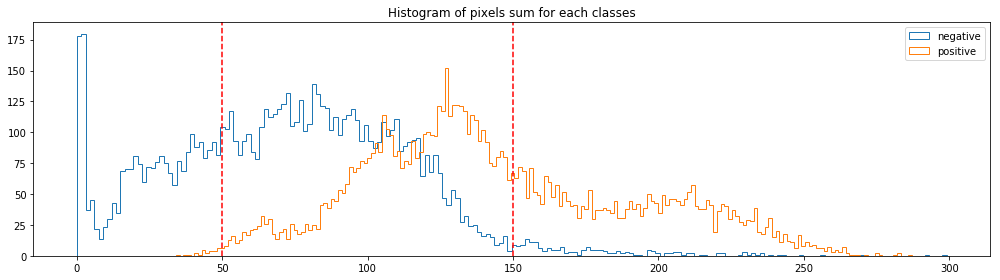
\includegraphics[width=1.0\textwidth]{images/pixels_hist}
    \caption{}
    \label{fig:pixels_hist}
\end{figure}

Na rysunku \ref{fig:pixels_sum_examples} pokazane są przykłady obrazków z zadanymi poziomami sumy pikseli. 

\begin{figure}[h!]
    \centering
    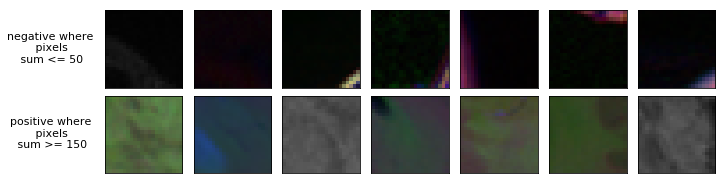
\includegraphics[width=1.0\textwidth]{images/pixels_sum_examples}
    \caption{}
    \label{fig:pixels_sum_examples}
\end{figure}

\section{Back to basic models}

\begin{figure}[h!]
    \centering
    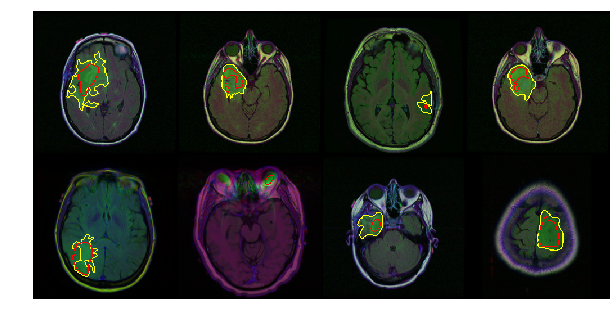
\includegraphics[width=1.0\textwidth]{images/logreg_mask}
    \caption{}
    \label{fig:logreg_mask}
\end{figure}

\begin{figure}[h!]
    \centering
    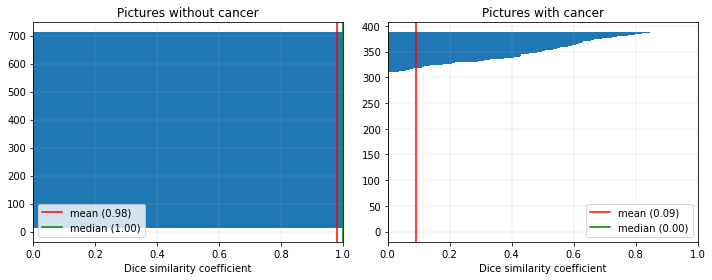
\includegraphics[width=1.0\textwidth]{images/logreg_dsc}
    \caption{}
    \label{fig:logreg_dsc}
\end{figure}

\begin{figure}[h!]
    \centering
    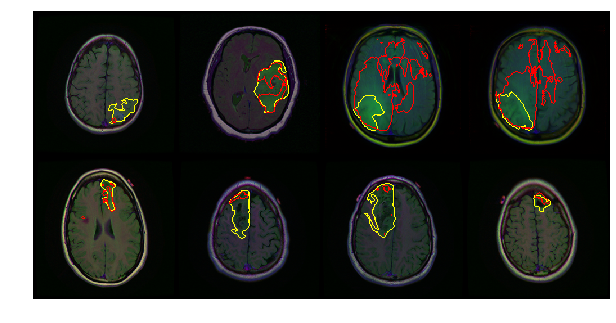
\includegraphics[width=1.0\textwidth]{images/simcnn_mask}
    \caption{}
    \label{fig:simcnn_mask}
\end{figure}

\begin{figure}[h!]
    \centering
    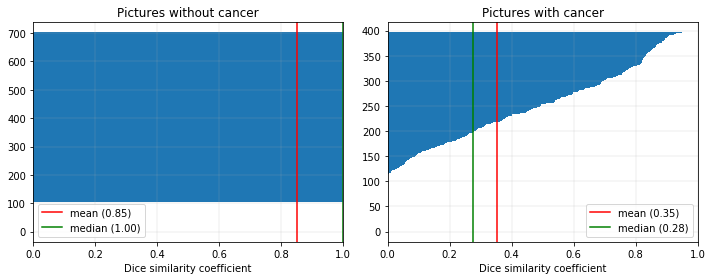
\includegraphics[width=1.0\textwidth]{images/simcnn_dsc}
    \caption{}
    \label{fig:simcnn_dsc}
\end{figure}



